\documentclass[]{article}
\usepackage[utf8]{inputenc}
\usepackage[sumlimits]{amsmath}
\usepackage{amssymb}
\usepackage{color,array,graphics}
\usepackage{hyperref}
\usepackage{enumerate}
\usepackage{graphicx}
\usepackage{amsmath, amsthm, amssymb}
\usepackage[shortlabels]{enumitem}
\usepackage[english]{babel}
\usepackage{tikz}
\usepackage{caption}
\usepackage{subcaption}
\usepackage{cellspace}
\setlength\cellspacetoplimit{4pt}
\setlength\cellspacebottomlimit{4pt}

\newcommand\cincludegraphics[2][]{\raisebox{-0.1\height}{\includegraphics[#1]{#2}}}

\setlength{\textheight}{8.5in}
\setlength{\textwidth}{6.5in}
\setlength{\oddsidemargin}{0in}
\setlength{\evensidemargin}{0in}
\voffset0.0in

\def\OR{\vee}
\def\AND{\wedge}
\def\imp{\rightarrow}
\def\math#1{$#1$}
\def\mand#1{$$#1$$}
\def\mld#1{\begin{equation}
#1
\end{equation}}
\def\eqar#1{\begin{eqnarray}
#1
\end{eqnarray}}
\def\eqan#1{\begin{eqnarray*}
#1
\end{eqnarray*}}
\def\cl#1{{\cal #1}}

\DeclareSymbolFont{AMSb}{U}{msb}{m}{n}
\DeclareMathSymbol{\N}{\mathbin}{AMSb}{"4E}
\DeclareMathSymbol{\Z}{\mathbin}{AMSb}{"5A}
\DeclareMathSymbol{\R}{\mathbin}{AMSb}{"52}
\DeclareMathSymbol{\Q}{\mathbin}{AMSb}{"51}
\DeclareMathSymbol{\I}{\mathbin}{AMSb}{"49}
\DeclareMathSymbol{\C}{\mathbin}{AMSb}{"43}

\title{Assignment 2}
\author{Batch Size of 3}

\begin{document}

\maketitle

\clearpage
\section{Improvement on the dataset}
We updated the dataset by incorporating new computer-rendered LEGO images, introducing diverse and expanded data. Unlike the previous dataset, which featured bricks with only slight hue variations, a null background and just bricks, the updated collection encompasses various LEGO classes, such as rectangular bricks, sloped bricks, plates, walls, and miscellaneous (irregular shapes). This new dataset accurately represents LEGO colors and incorporates realistic shading, accompanied by a dynamic background featuring both diffuse and glossy spots. Furthermore, we've introduced increased variability in lighting conditions and camera angles. \\

\begin{figure}[h]
    \centering
    \begin{subfigure}[b]{0.2\textwidth}
        \centering
        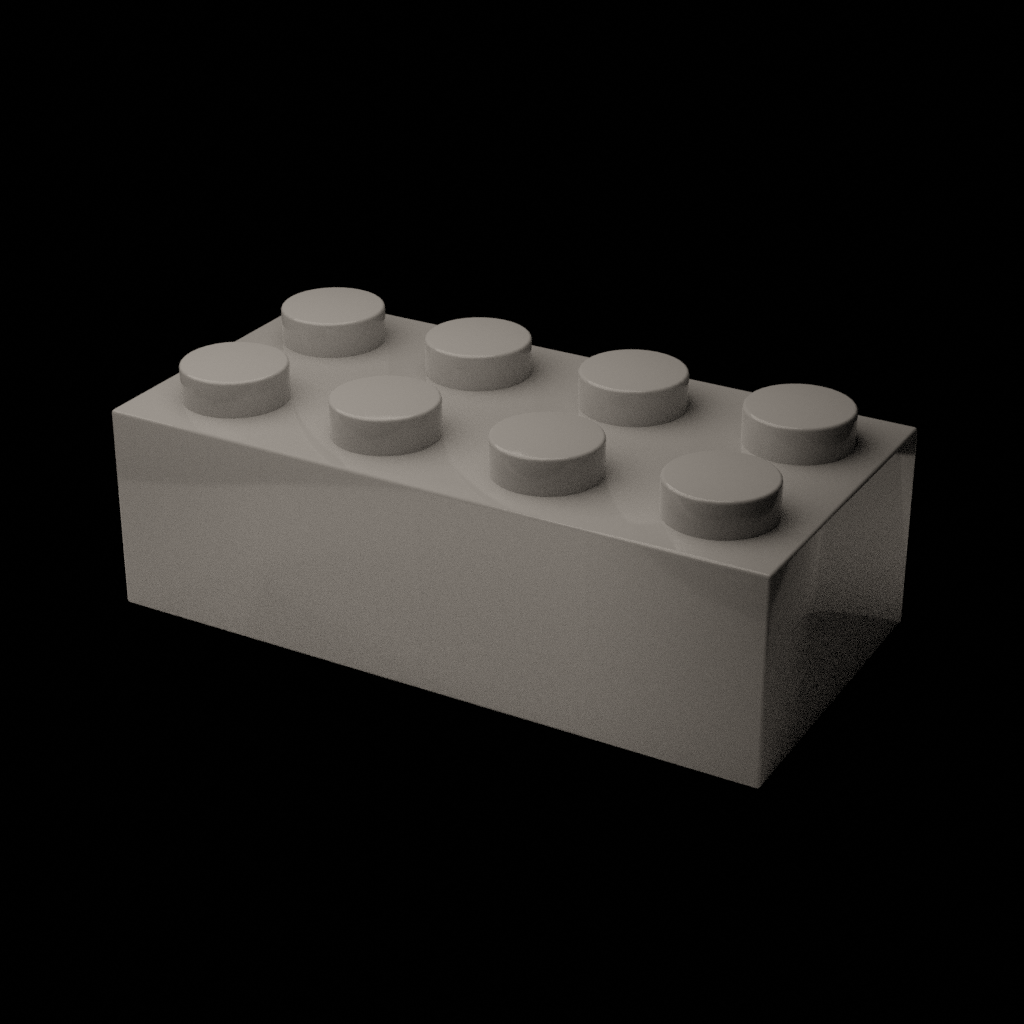
\includegraphics[width=\textwidth]{single example/oldex.png}
        \caption{Old Data Example}
    \end{subfigure}
    \begin{subfigure}[b]{0.2\textwidth}
        \centering
        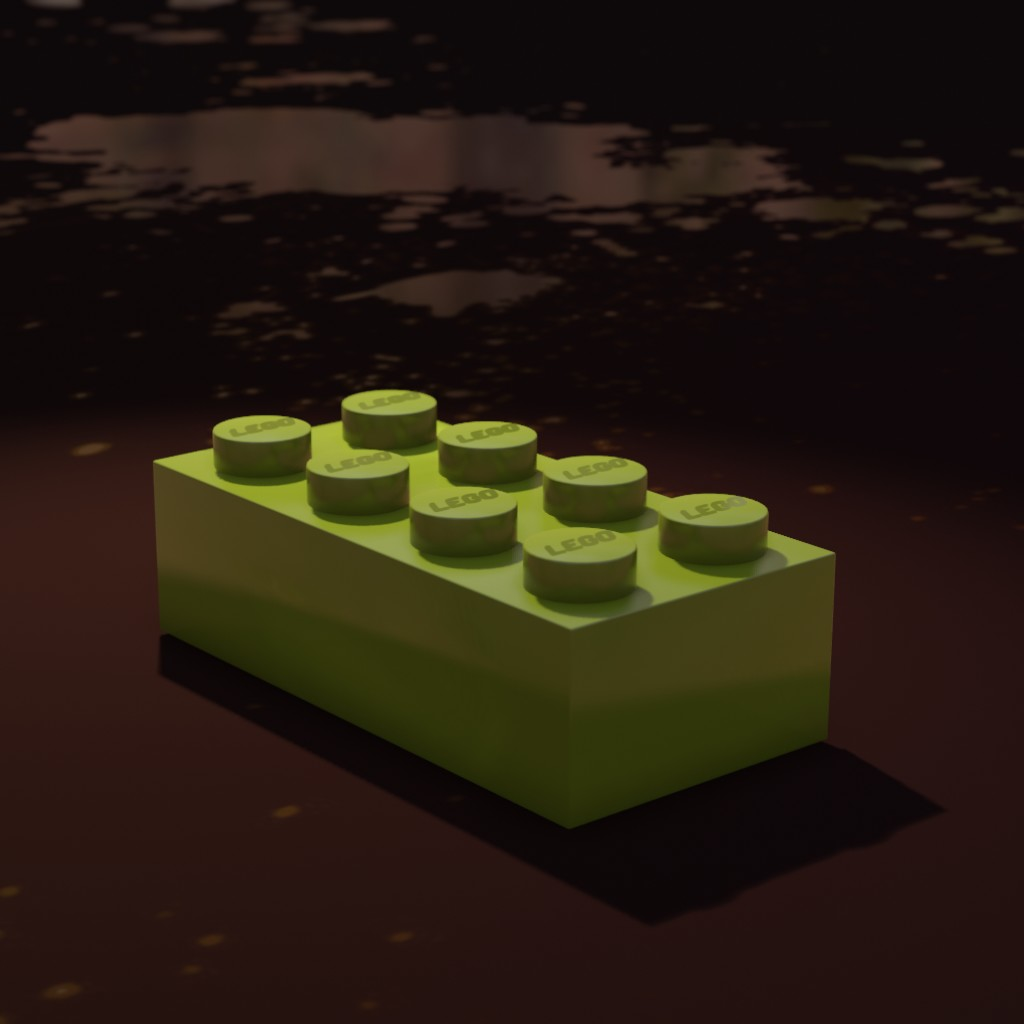
\includegraphics[width=\textwidth]{single example/newex.jpg}
        \caption{New Data Example}
    \end{subfigure}
    \begin{subfigure}[b]{0.4\textwidth}
        \centering
        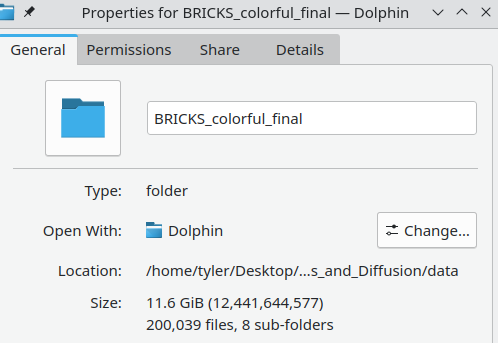
\includegraphics[width=\textwidth]{dataset.png}
        \caption{Dataset}
    \end{subfigure}\par\medskip
\end{figure}

In our new dataset, we included 10,000 to 20,000 images of each category for a class. Our dataset includes a class (i.e. bricks, plates, slopes), and a category of the class (i.e. brick-1x1, slope-1x2). Note that some files have some extra images.
\begin{verbatim}
\dataset (200,000 datapoints)
    \bricks (40,000)
        - bricks-1x1 (10,000 images)
        - bricks-1x2 (10,000 images)
        - bricks-2x2 (8,000 images)
        - bricks-2x4 (12,000 images)
    \miscellaneous (30,000)
        - arch-1 (10,000 images)
        - fence (10,000 images)
        - flags (10,000 images)
    \plates (40,000)
        - plate-1x1 (10,000 images)
        - plate-1x2 (10,000 images)
        - plate-2x2 (10,000 images)
        - plate-2x4 (10,000 images)
    \slopes (60,000)
        - slope-1x2 (20,000 images)
        - slope-2x2 (20,000 images)
        - slope-2x4 (20,000 images)
    \wall (30,000)
        - wall-2 (10,000 images)
        - wall-4 (10,000 images)
        - wall-6 (10,000 images)
\end{verbatim}

\begin{figure}[h]
    \centering
    \begin{subfigure}[b]{0.15\textwidth}
        \centering
        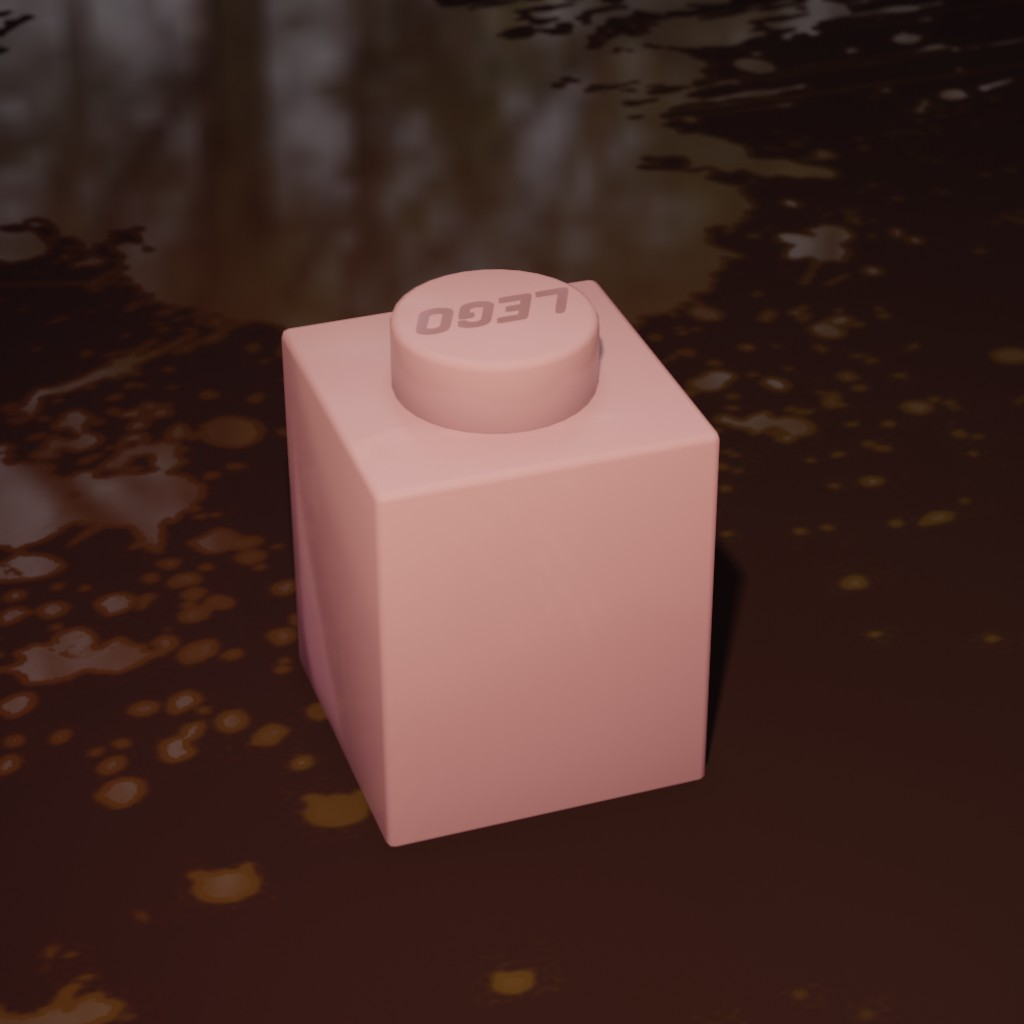
\includegraphics[width=\textwidth]{Examples/bricks-1x1.jpg}
        \caption{Brick 1x1}
    \end{subfigure}
    \begin{subfigure}[b]{0.15\textwidth}
        \centering
        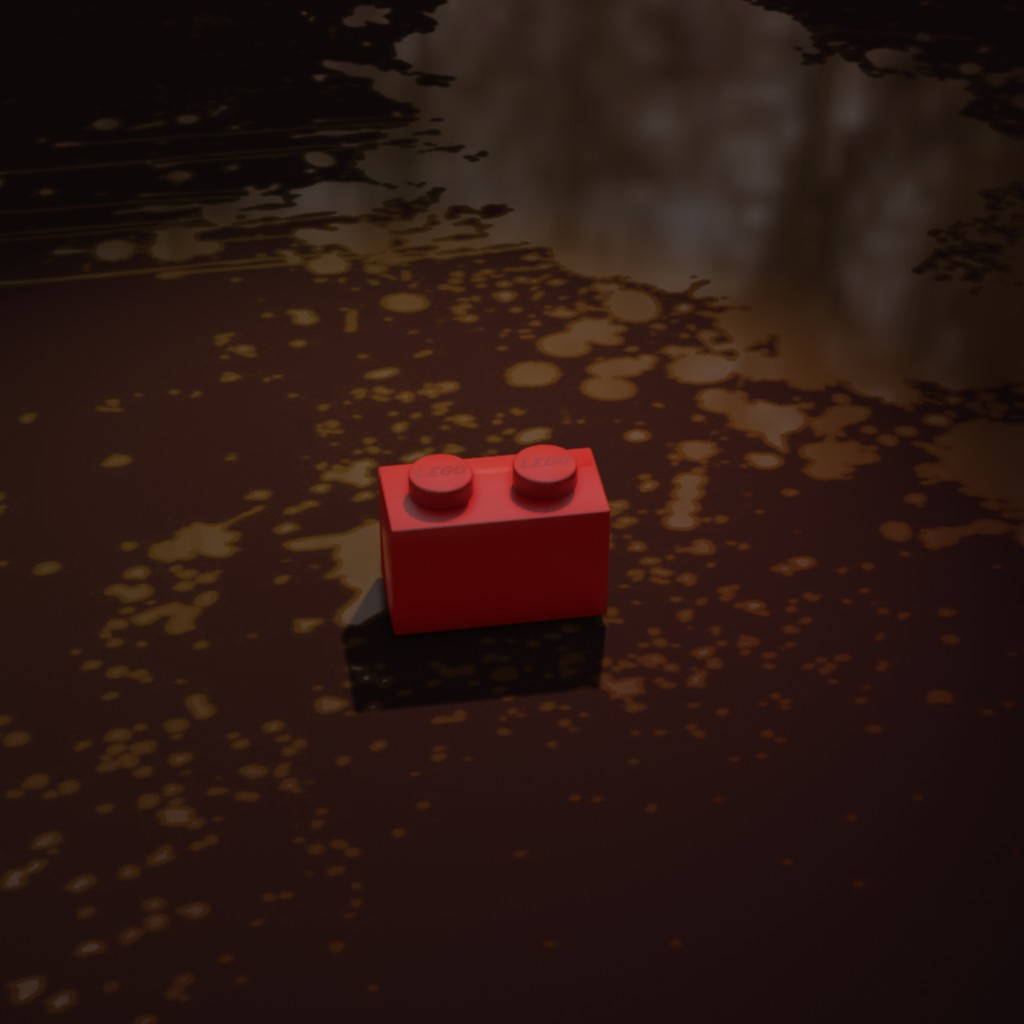
\includegraphics[width=\textwidth]{Examples/bricks-1x2.jpg}
        \caption{Brick 1x2}
    \end{subfigure}
    \begin{subfigure}[b]{0.15\textwidth}
        \centering
        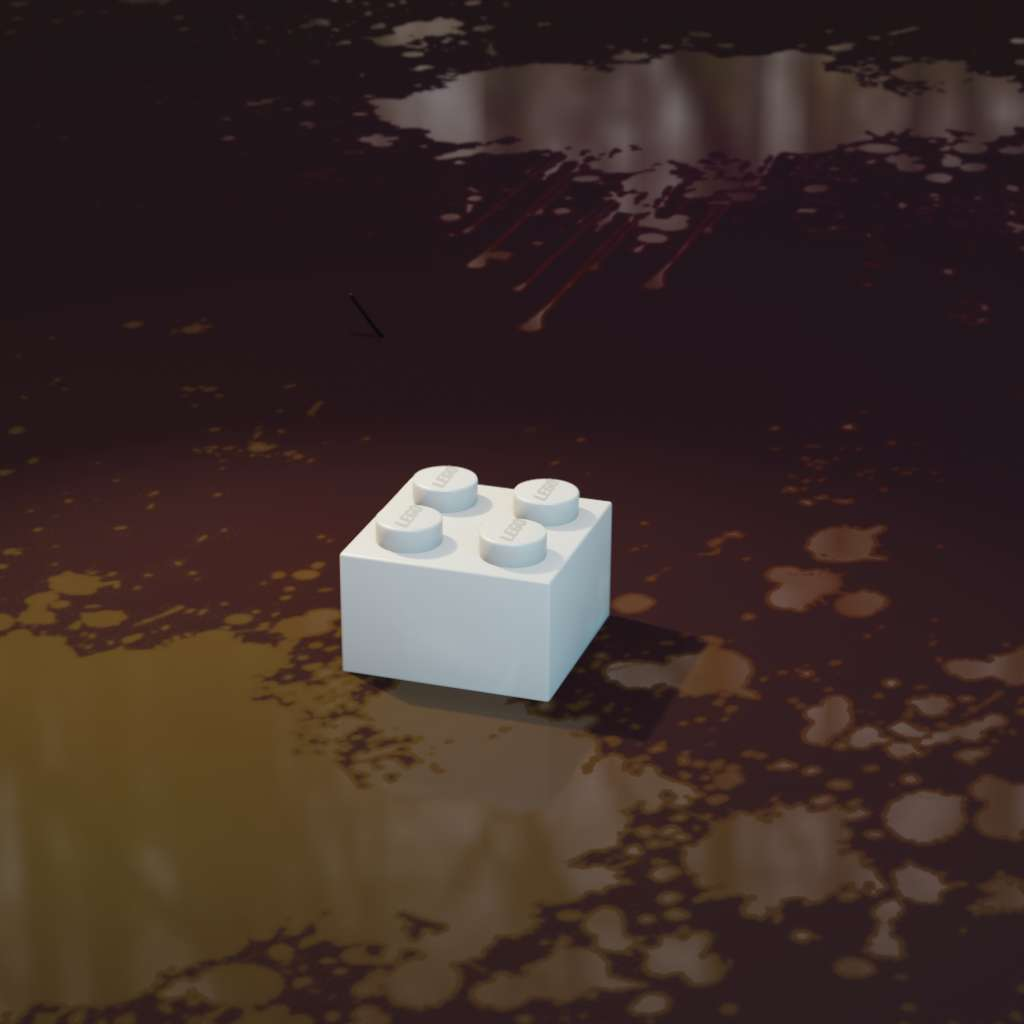
\includegraphics[width=\textwidth]{Examples/bricks-2x2.jpg}
        \caption{Brick 2x2}
    \end{subfigure}
    \begin{subfigure}[b]{0.15\textwidth}
        \centering
        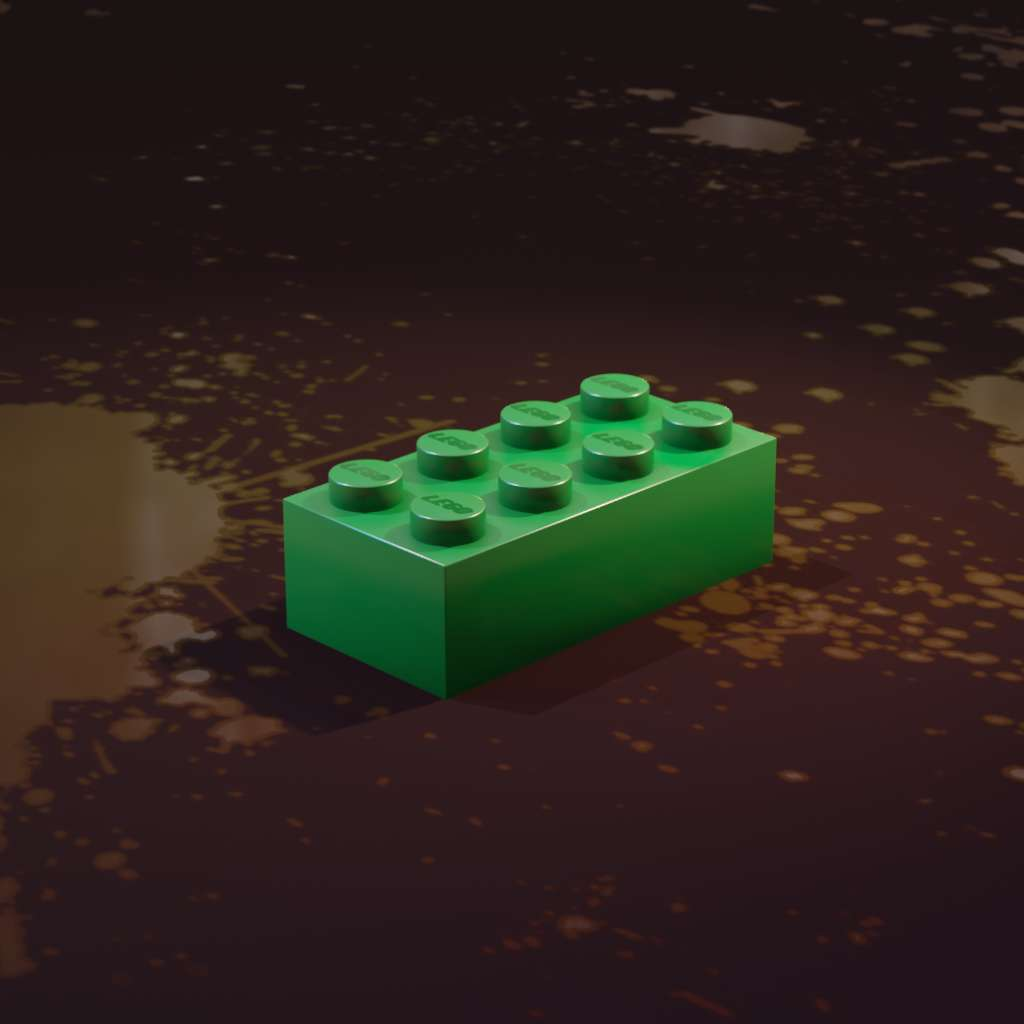
\includegraphics[width=\textwidth]{Examples/bricks-2x4.jpg}
        \caption{Brick 2x4}
    \end{subfigure}
    \begin{subfigure}[b]{0.15\textwidth}
        \centering
        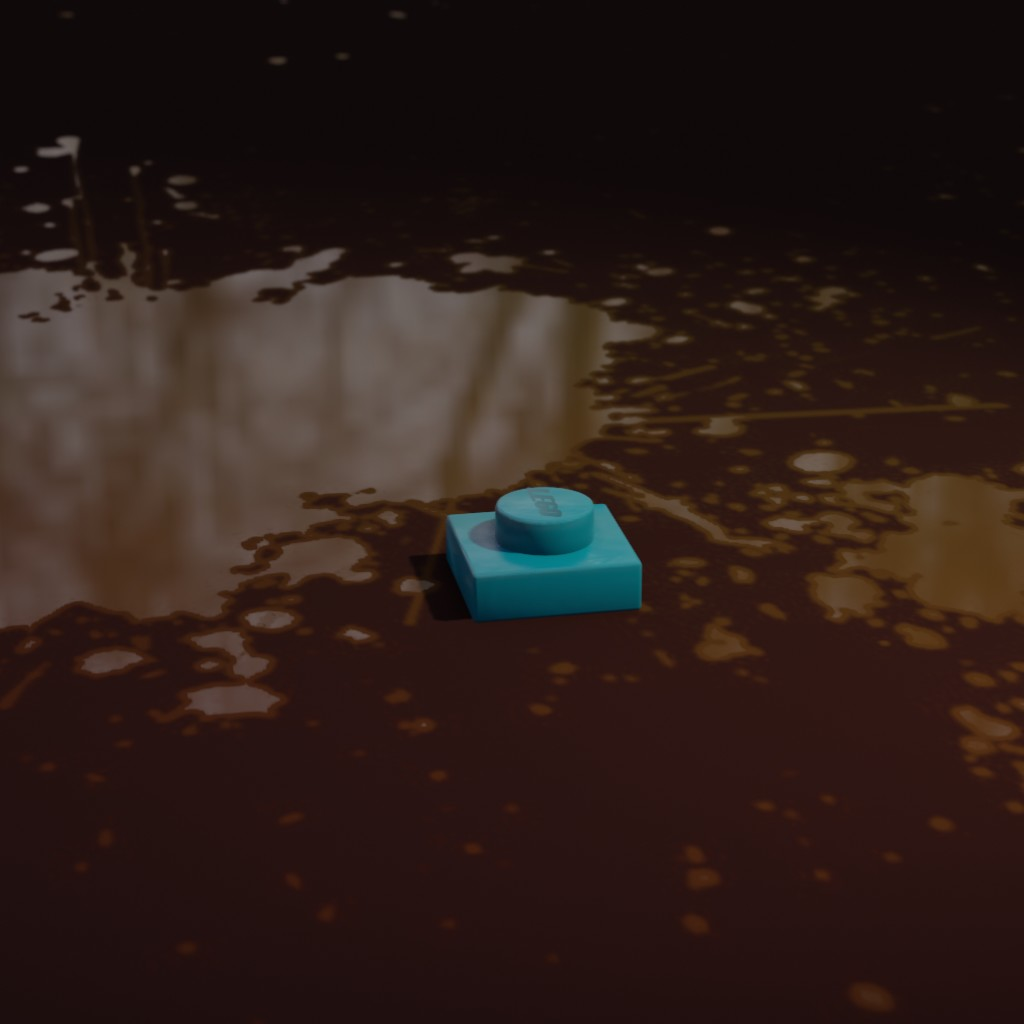
\includegraphics[width=\textwidth]{Examples/plate-1x1.jpg}
        \caption{Plate 1x1}
    \end{subfigure}\par\medskip
    \begin{subfigure}[b]{0.15\textwidth}
        \centering
        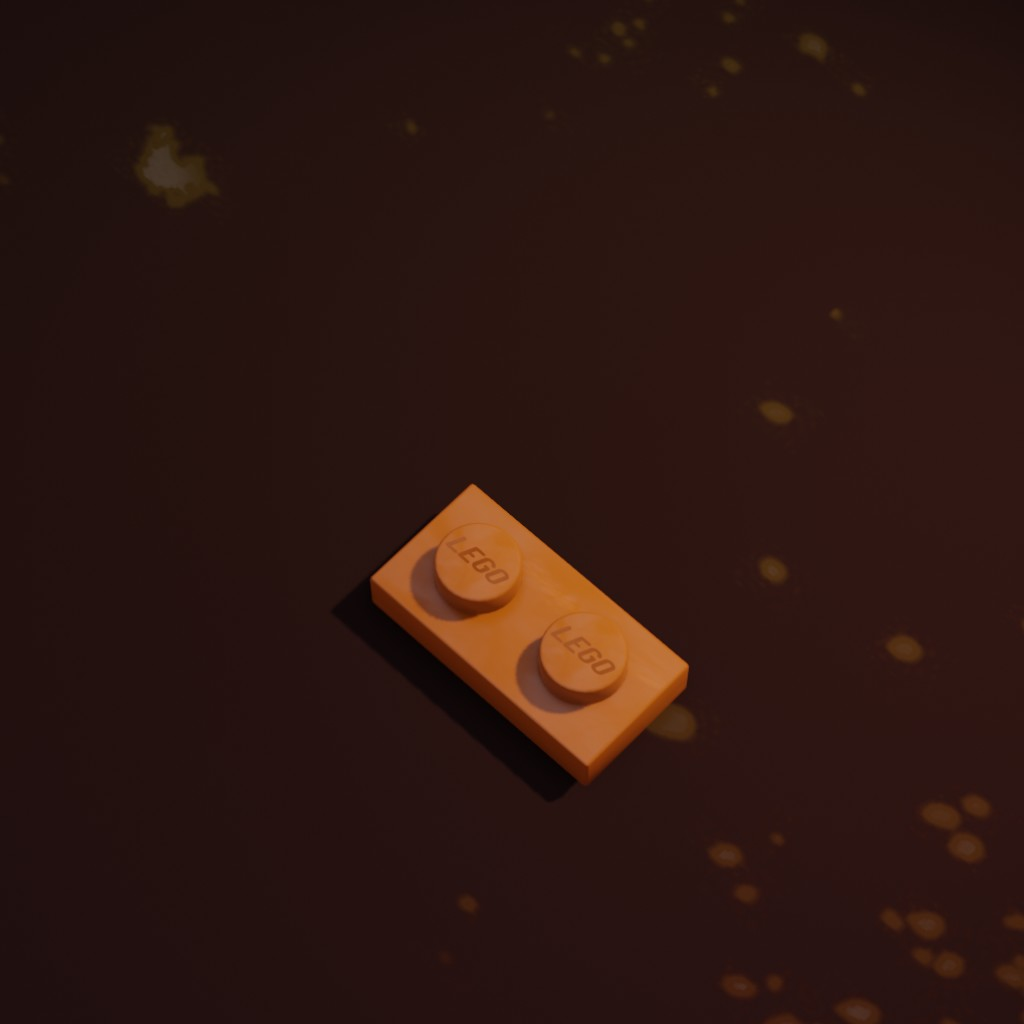
\includegraphics[width=\textwidth]{Examples/plate-1x2.jpg}
        \caption{Plate 1x2}
    \end{subfigure}
    \begin{subfigure}[b]{0.15\textwidth}
        \centering
        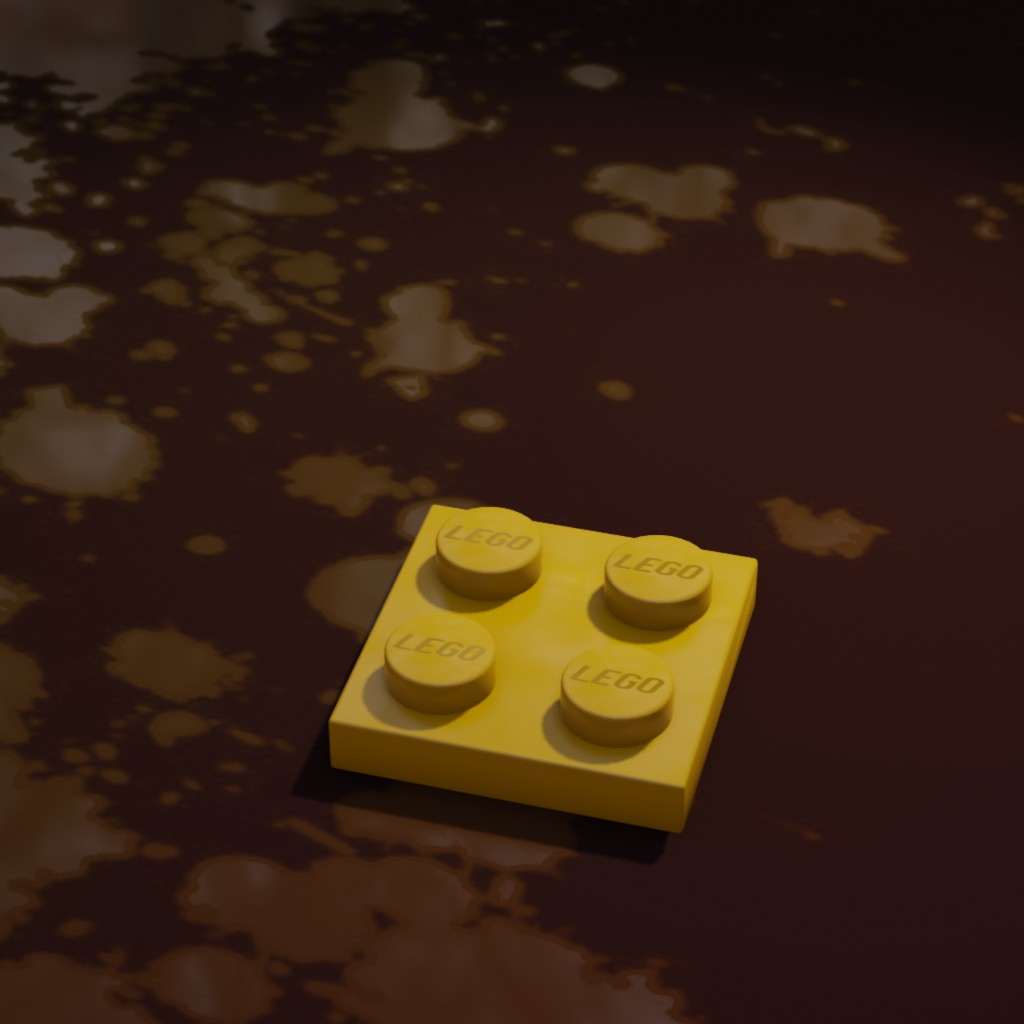
\includegraphics[width=\textwidth]{Examples/plate-2x2.jpg}
        \caption{Plate 2x2}
    \end{subfigure}
    \begin{subfigure}[b]{0.15\textwidth}
        \centering
        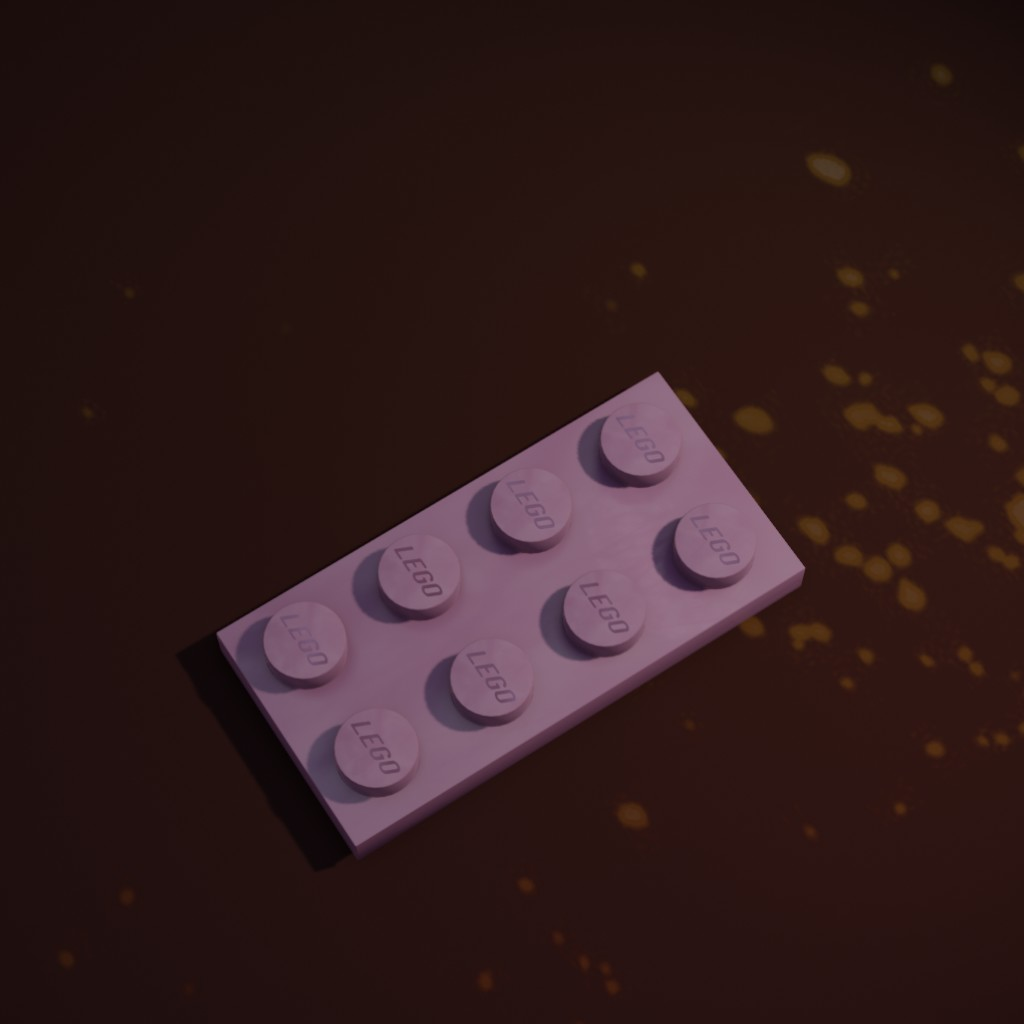
\includegraphics[width=\textwidth]{Examples/plate-2x4.jpg}
        \caption{Plate 2x4}
    \end{subfigure}
    \begin{subfigure}[b]{0.15\textwidth}
        \centering
        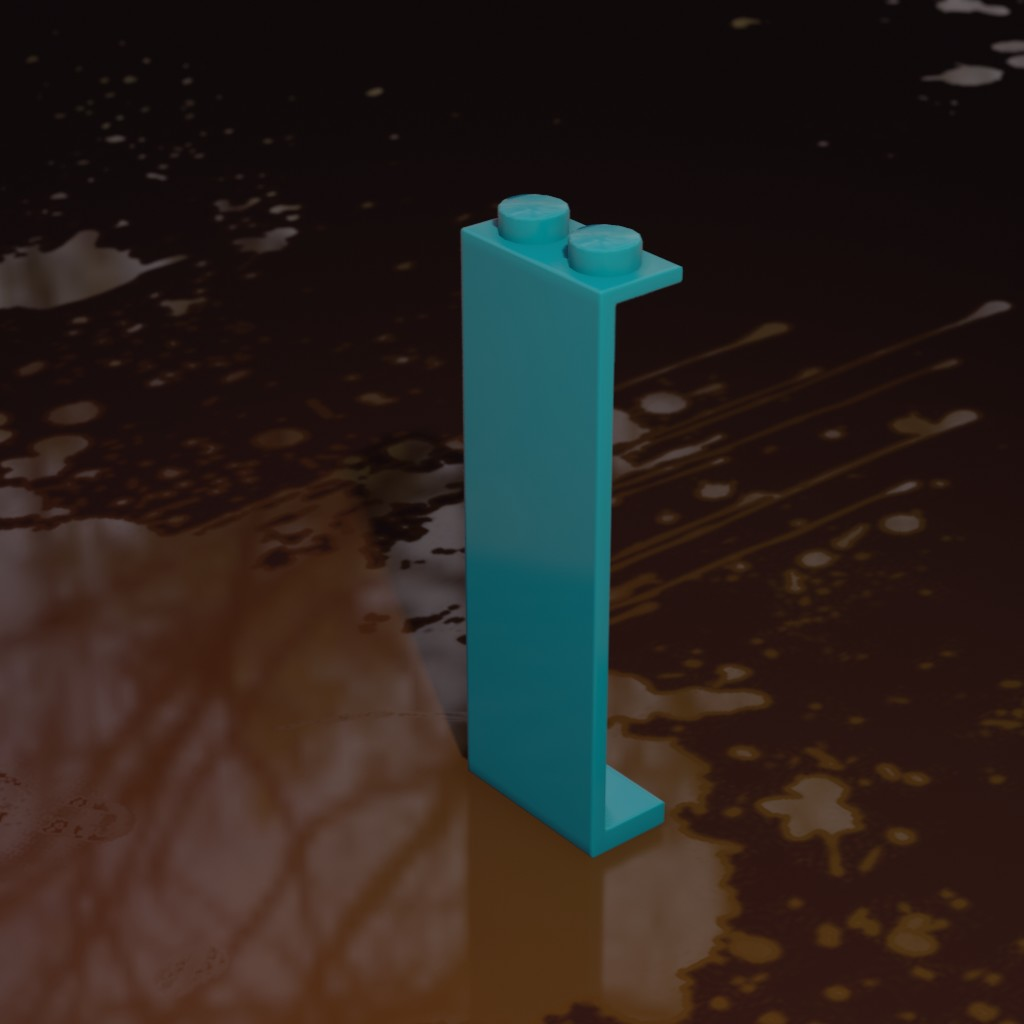
\includegraphics[width=\textwidth]{Examples/wall-2.jpg}
        \caption{Wall 2}
    \end{subfigure}
    \begin{subfigure}[b]{0.15\textwidth}
        \centering
        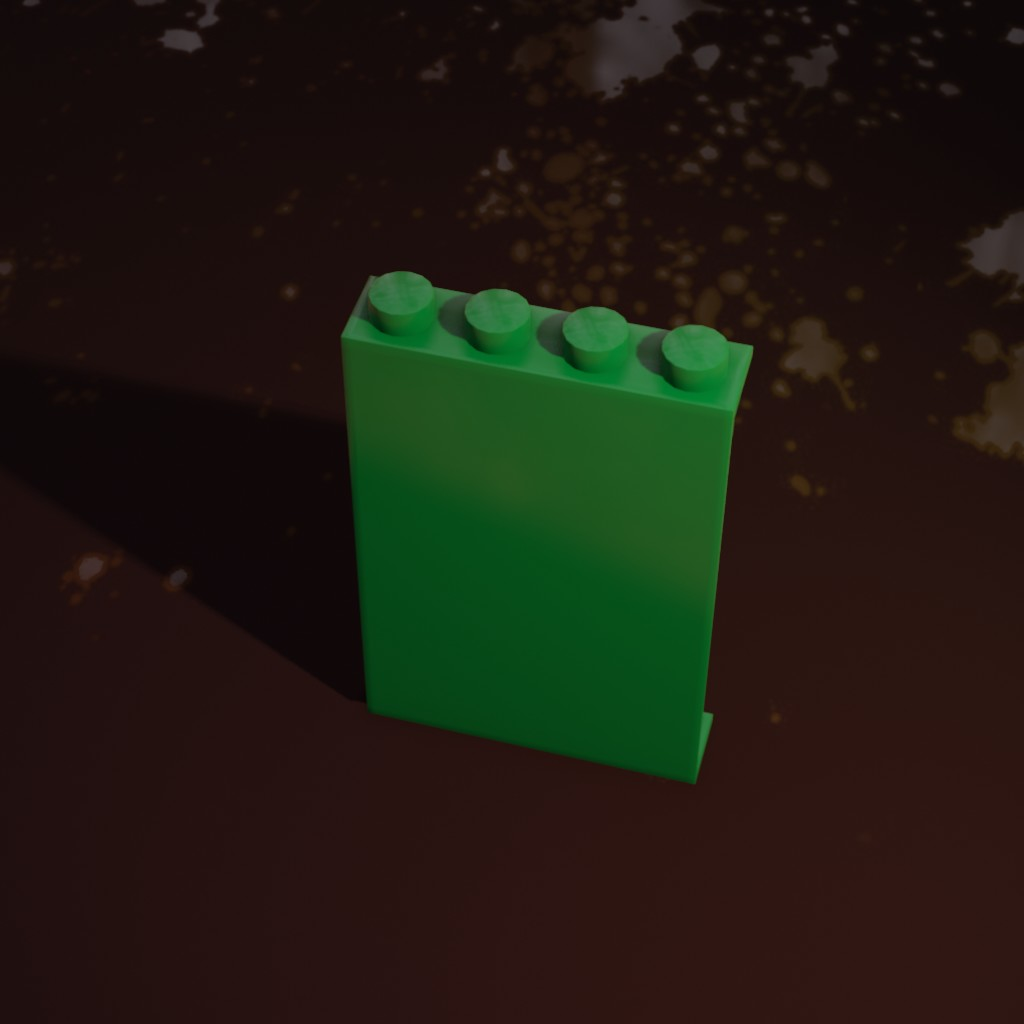
\includegraphics[width=\textwidth]{Examples/wall-4.jpg}
        \caption{Wall 4}\par\medskip
    \end{subfigure}\par\medskip
    \begin{subfigure}[b]{0.15\textwidth}
        \centering
        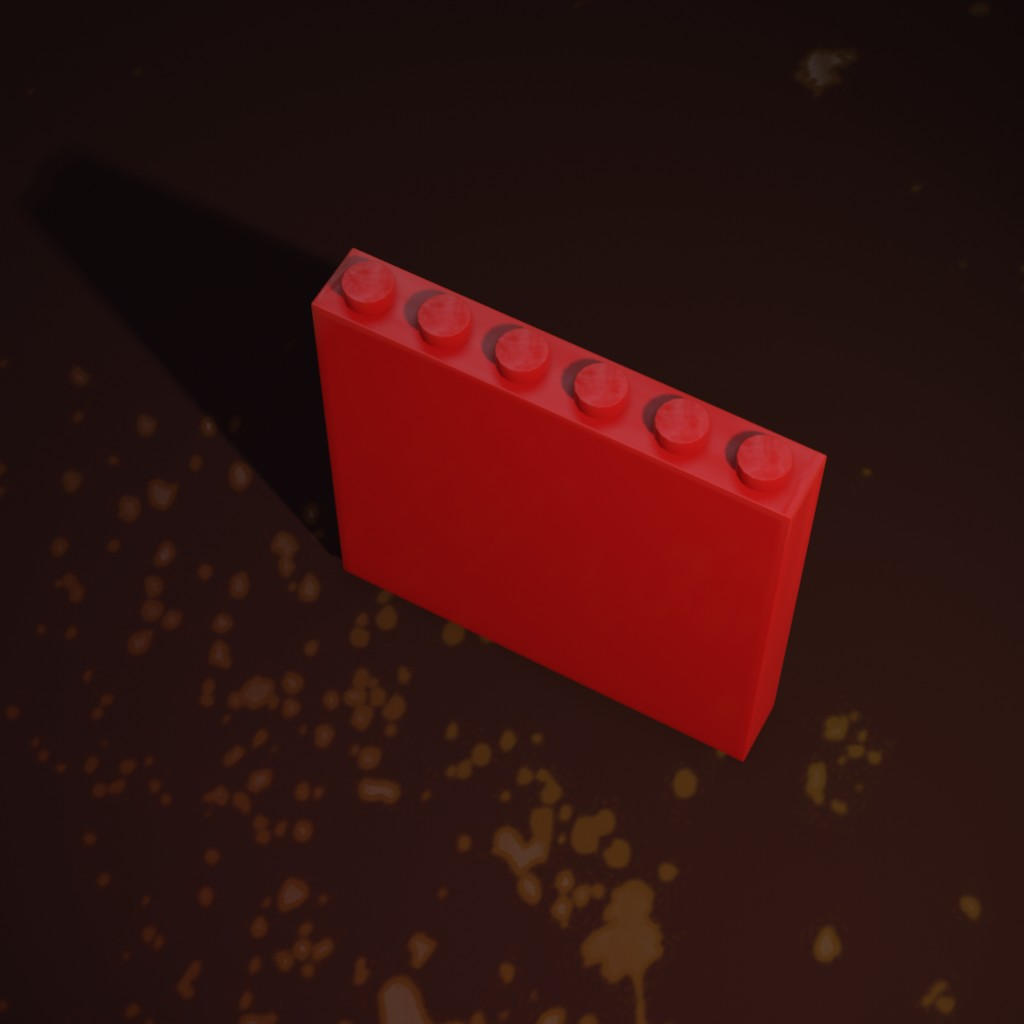
\includegraphics[width=\textwidth]{Examples/wall-6.jpg}
        \caption{Wall 6}
    \end{subfigure}
    \begin{subfigure}[b]{0.15\textwidth}
        \centering
        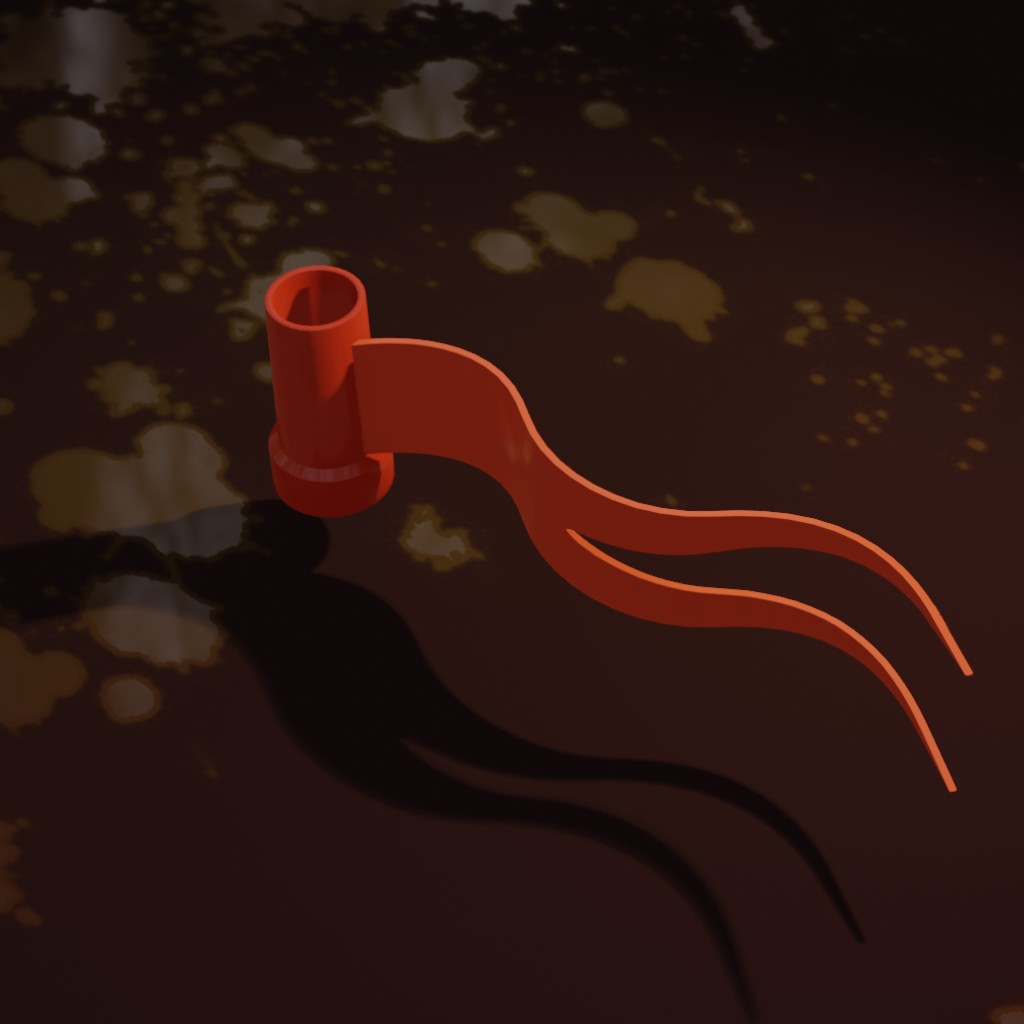
\includegraphics[width=\textwidth]{Examples/flag.jpg}
        \caption{Flag}
    \end{subfigure}
    \begin{subfigure}[b]{0.15\textwidth}
        \centering
        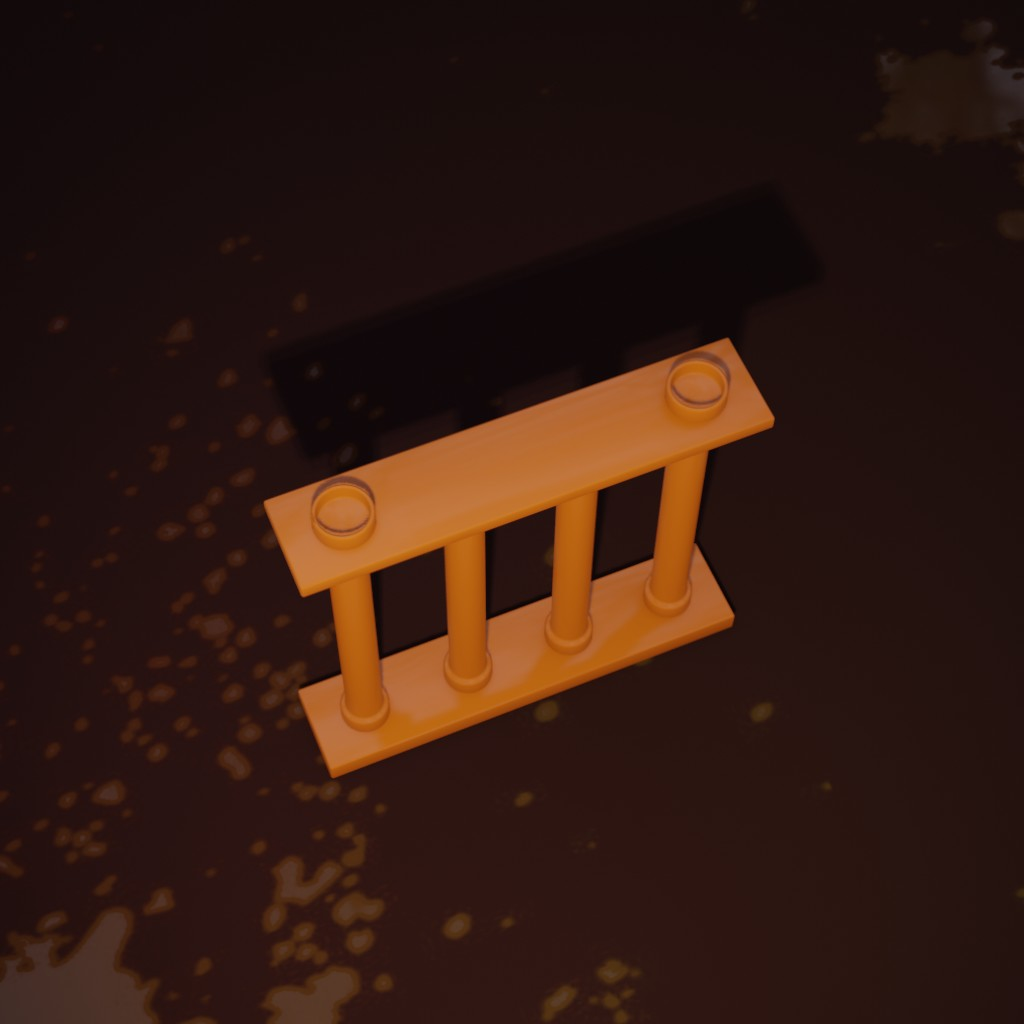
\includegraphics[width=\textwidth]{Examples/fence.jpg}
        \caption{Fence}
    \end{subfigure}
    \begin{subfigure}[b]{0.15\textwidth}
        \centering
        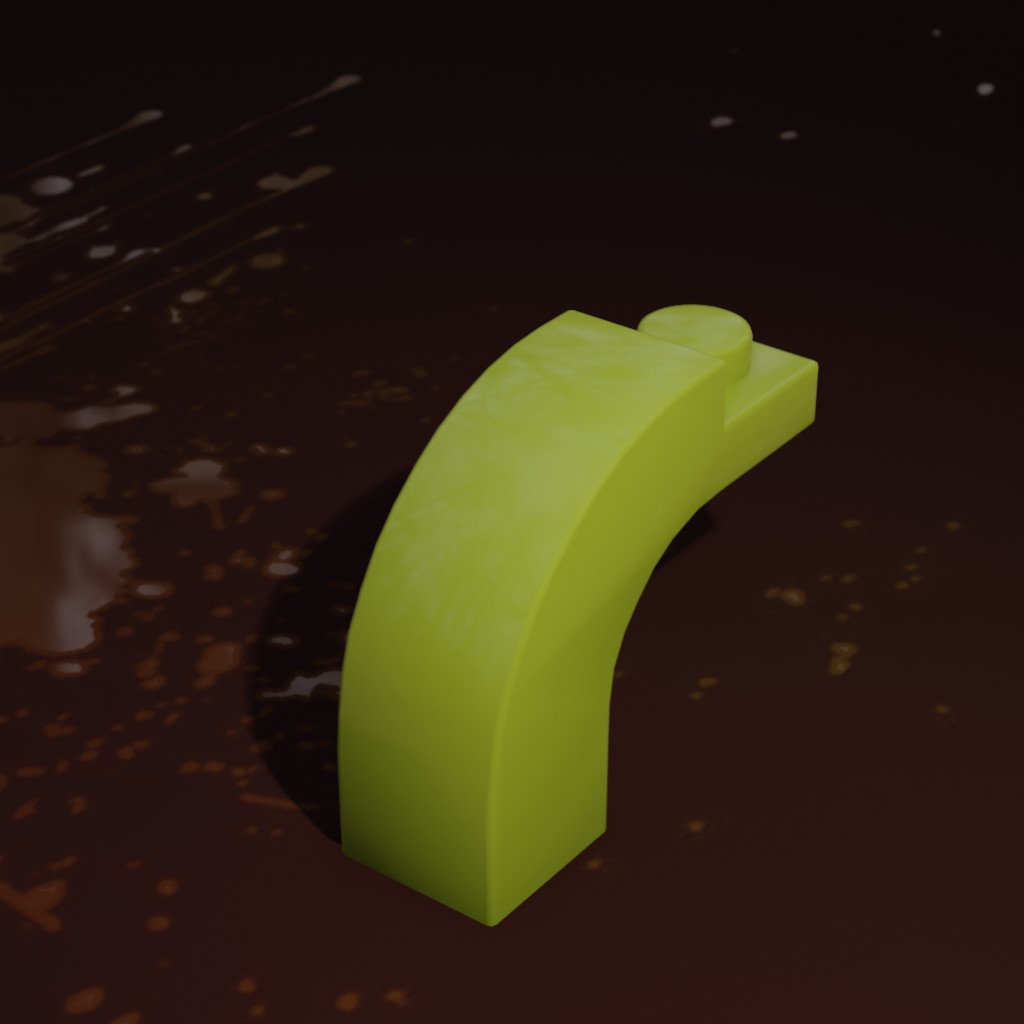
\includegraphics[width=\textwidth]{Examples/arch-1.jpg}
        \caption{Arch 1}\par\medskip
    \end{subfigure}
    \begin{subfigure}[b]{0.15\textwidth}
        \centering
        
\includegraphics[width=\textwidth]{Examples/slope-1x2.jpg}
        \caption{Slope 1x2}\par\medskip
    \end{subfigure}\par\medskip
    \begin{subfigure}[b]{0.15\textwidth}
        \centering
        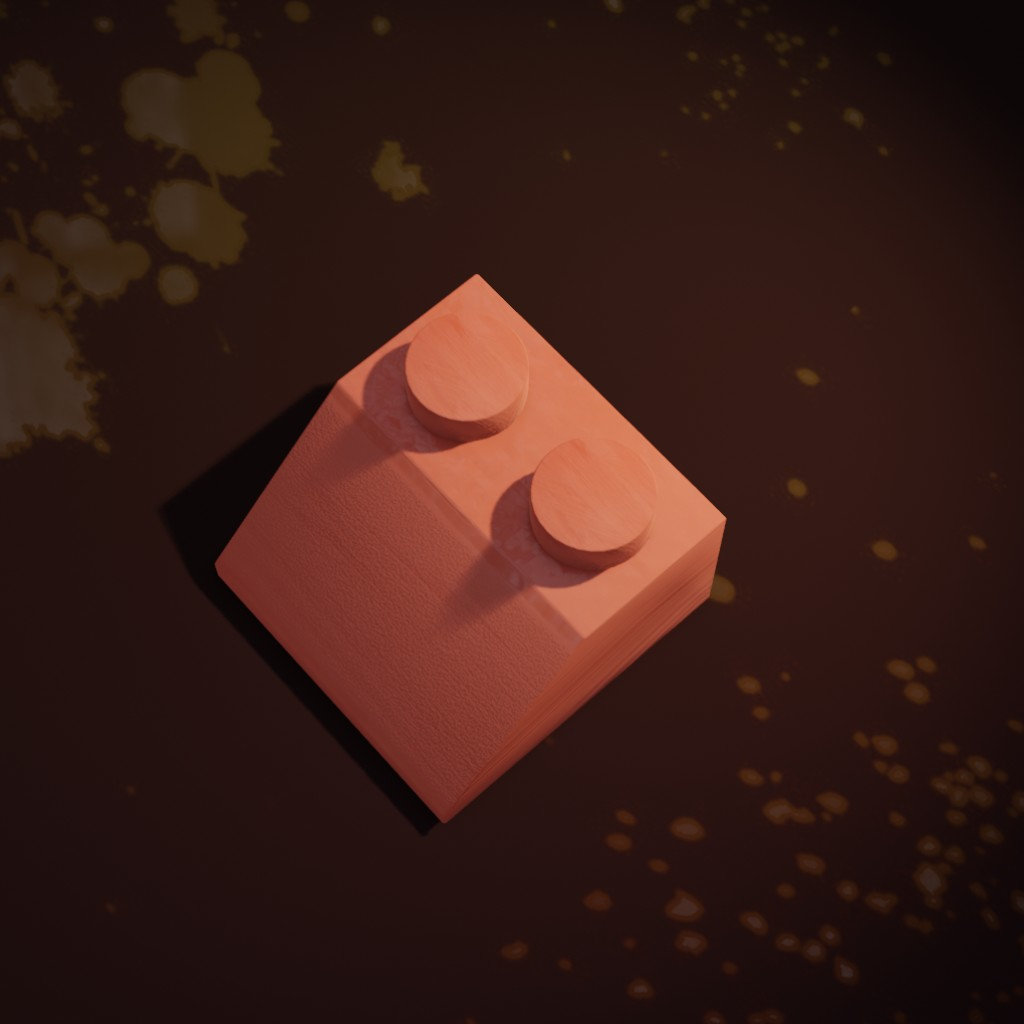
\includegraphics[width=\textwidth]{Examples/slope-2x2.jpg}
        \caption{Slope 2x2}\par\medskip
    \end{subfigure}
    \begin{subfigure}[b]{0.15\textwidth}
        \centering
        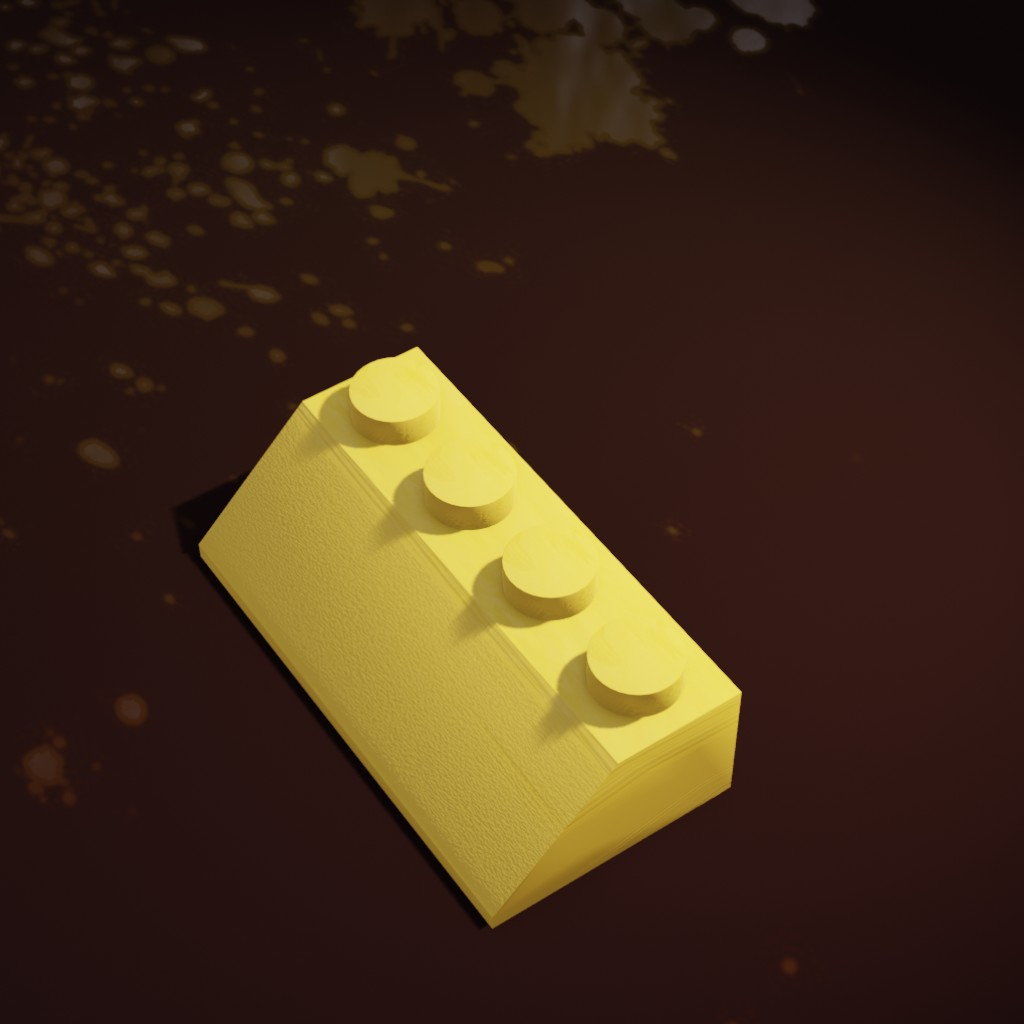
\includegraphics[width=\textwidth]{Examples/slope-2x4.jpg}
        \caption{Slope 2x4}\par\medskip
    \end{subfigure}
    \caption{Examples of our dataset}
\end{figure}

\begin{figure}[h]
    \centering
    \begin{subfigure}[b]{0.25\textwidth}
        \centering
        
\includegraphics[width=\textwidth]{colors/brick-plate-colors.png}
        \caption{Brick and Plate}
    \end{subfigure}\par\medskip
    \begin{subfigure}[b]{0.25\textwidth}
        \centering
        
\includegraphics[width=\textwidth]{colors/fence-colors.png}
        \caption{Fence}
    \end{subfigure}\par\medskip
    \begin{subfigure}[b]{0.25\textwidth}
        \centering
        
\includegraphics[width=\textwidth]{colors/slope-colors.png}
        \caption{Slope}
    \end{subfigure}\par\medskip
    \caption{Color gradient for LEGO pieces}
\end{figure}

\clearpage

\section{Degree of Similarity}

\begin{tabular}{cc}
    \begin{minipage}{0.2\linewidth}
        \begin{tabular}{| Sc | }
            \hline
          Original Images \\
          \hline
          1 \cincludegraphics[height=1.5cm]{random-bricks/1.jpg} \\
          \hline
          2 \cincludegraphics[height=1.5cm]{random-bricks/2.jpg}  \\
          \hline
          3 \cincludegraphics[height=1.5cm]{random-bricks/3.jpg} \\
          \hline
          4 \cincludegraphics[height=1.5cm]{random-bricks/4.jpg} \\
          \hline
          5 \cincludegraphics[height=1.5cm]{random-bricks/5.jpg} \\
          \hline
          6 \cincludegraphics[height=1.5cm]{random-bricks/6.jpg}  \\
          \hline
          7 \cincludegraphics[height=1.5cm]{random-bricks/7.jpg} \\
          \hline
          8 \cincludegraphics[height=1.5cm]{random-bricks/8.jpg} \\
          \hline
          9 \cincludegraphics[height=1.5cm]{random-bricks/9.jpg} \\
          \hline
          10 \cincludegraphics[height=1.5cm]{random-bricks/10.jpg}\\
          \hline
        \end{tabular}
    \end{minipage} &
    \begin{minipage}{\linewidth}
        \begin{tabular}{| Sc |c |c |c | c | c | c |}
            \hline
          Compared Pairs (with aug) & LPIPS & MSE & SSIM & Tyler & Zhi & Alan\\
          \hline
          \cincludegraphics[height=4cm]{MLE SSIM/110.png} & 0.491 & 0.01 & 0.82 & 0.4 & 0.3 & 0.6\\
          \hline
          \cincludegraphics[height=4cm]{MLE SSIM/210.png} & 0.528 & 0.02 & 0.78 & 0.6 & 0.7 & 0.6\\
          \hline
          \cincludegraphics[height=4cm]{MLE SSIM/23.png} & 0.528 & 0.02 & 0.78 & 0.5 & 0.4 & 0.4\\
          \hline
          \cincludegraphics[height=4cm]{MLE SSIM/34.png} & 0.522 & 0.03 & 0.81 & 0.8 & 1.0 & 1.0\\
          \hline
        \end{tabular}
    \end{minipage} 
\end{tabular}

\begin{tabular}{| Sc |c | c | c | c | c | c |}
        \hline
          Compared Pairs (with aug) & LPIPS & MSE & SSIM & Tyler & Zhi & Alan\\
          \hline
          \cincludegraphics[height=4cm]{MLE SSIM/45.png} & 0.550 & 0.05 & 0.66 & 0.8 & 0.9 & 1.0\\
        \hline
        \cincludegraphics[height=4cm]{MLE SSIM/56.png} & 0.473 & 0.04 & 0.70 & 0.8 & 0.7 & 1.0\\
        \hline
        \cincludegraphics[height=4cm]{MLE SSIM/67.png} & 0.474 & 0.03 & 0.75 & 0.4 & 0.7 & 0.6\\
        \hline
        \cincludegraphics[height=4cm]{MLE SSIM/78.png} & 0.559 & 0.02 & 0.79 & 0.6 & 0.6 & 0.6\\
        \hline
        \cincludegraphics[height=4cm]{MLE SSIM/89.png} & 0.569 & 0.03 & 0.78 & 0.8 & 1.0 & 0.8\\
        \hline
\end{tabular}

\textbf{Only from "Compared Pairs (with aug)"}
\begin{itemize}
    \item Average MSE: 0.025, Average SSIM: 0.687
    \item Average LPIPS: 0.52127 +/- 0.01112
    \item Average Tyler: 0.55
    \item Average Zhi: 0.63
    \item Average Alan: 0.68
\end{itemize}
\subsection*{All comparisons from Tyler/Alan/Zhi}
\begin{tabular}{|c|c|c|c|c|c|c|c|c|c|}
    \hline
    First Image/Second Image & 2 & 3 & 4 & 5 & 6 & 7 & 8 & 9 & 10\\
    \hline
    1 & 8/10/8 & 4/6/4 & 4/8/5 & 4/6/4 & 4/6/3 & 6/4/5 & 6/6/5 & 8/8/7 & 6/6/3 \\
    \hline
    2 && 4/4/4 & 4/4/3 & 4/4/3 & 4/4/3 & 6/4/6 & 6/4/5 & 6/4/5 & 6/6/7 \\
    \hline
    3 &&& 8/10/10 & 8/10/8 & 8/10/8 & 4/8/7 & 4/6/5 & 4/6/6 & 6/8/7 \\
    \hline
    4 &&&& 8/10/9 & 8/10/9 & 4/8/6 & 4/6/5 & 6/8/8 & 4/6/3 \\
    \hline
    5 &&&&& 8/10/7 & 4/6/6 & 4/6/5 & 4/6/6 & 4/6/3 \\
    \hline
    6 &&&&&& 4/6/7 & 4/6/5 & 4/6/3 & 4/6/4\\
    \hline
    7 &&&&&&& 6/6/6 & 6/6/7 & 6/6/7 \\
    \hline
    8 &&&&&&&& 8/8/9 & 8/10/7 \\
    \hline
    9 &&&&&&&&& 8/10/9 \\
    \hline
\end{tabular} 
\\ \\

If we example all of the results for the similarity, we can definitely say that for all situations MSE is not effective at all with our dataset. This is due to the fact that MSE compares every pixel value, which will always be different in this case since we have noise in the background with different colored legos in different rotations and locations. By looking at SSIM and LPIPS we have a more concrete comparison to a human similarity. \\
\\
On average, we can say that the human similarities are very close to each other. However, one person's average is closer to one comparison than the other, on one hand Alan's average is closer to SSIM, on the other hand Tyler's average is closer to LPIPS. \\

\clearpage
\begin{center}
    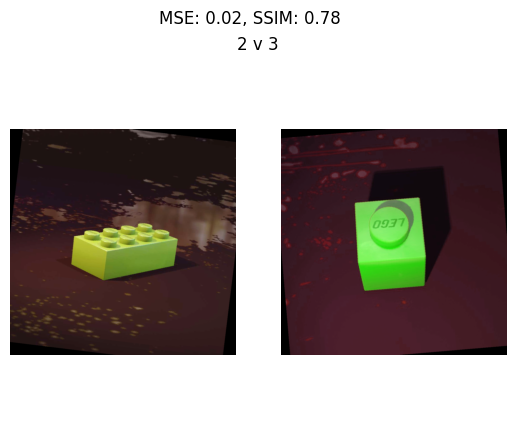
\includegraphics[width=6cm]{MLE SSIM/23.png}
\end{center}
\begin{itemize}
\item
    \textbf{LPIPS agree with human}: In the case of (2 v 3), the measurement given by LPIPS (0.528) agree more with the human similarity (around 0.5) than SSIM, which gave it a very high similarity score of 0.78. Having a lower similarity here makes sense, the two pieces are at a different angle, the color is different, and the shape is different.\\
    \begin{center}
        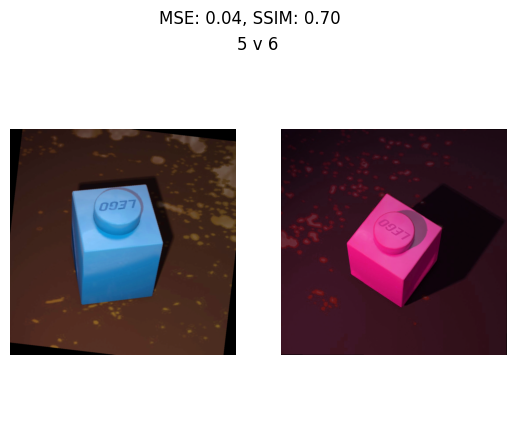
\includegraphics[width=6cm]{MLE SSIM/56.png}
    \end{center}
\item
    \textbf{SSIM agree with human}: In the case of (5 v 6), the measurement given by SSIM agree more with the human similarity (around 0.85) than LPIPS, which gave it a lower similarity score of (0.473). If we examine the two images, we can see that the rotation is only slightly off with the color changed, thus the two legos are very alike in that case. Thus, having a higher similarity score would make sense for these two images.\\
    \clearpage
    \begin{center}
        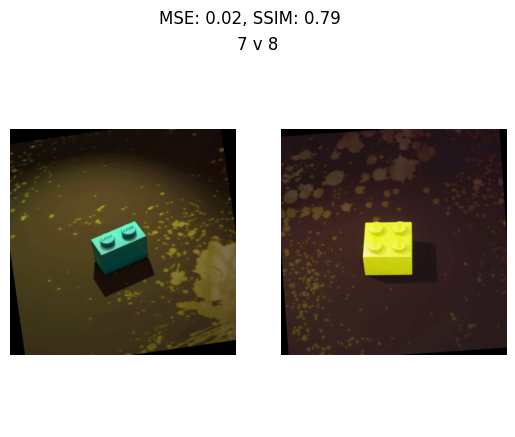
\includegraphics[width=6cm]{MLE SSIM/78.png}
    \end{center}
\item
    \textbf{Both agree with human}: In the case of (7 v 8), the measurement given by both SSIM, LPIPS, and the humans are mostly around the same, although SSIM is slightly higher than the rest. Regardless, the two pieces although different, show that they are close by a similar color and size relative to the viewer.\\
    \begin{center}
        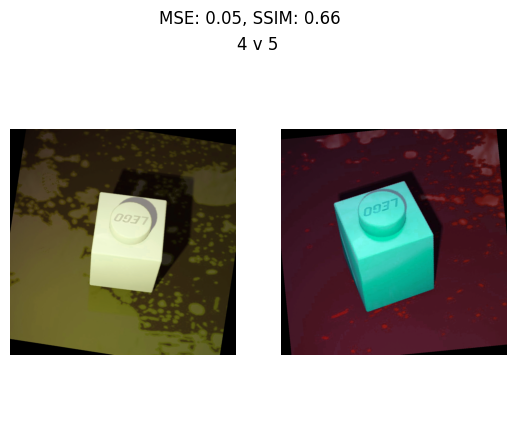
\includegraphics[width=6cm]{MLE SSIM/45.png}
    \end{center}
\item
    \textbf{Both disagree with human}: In the case of (4 v 5), we can say that on average, the human similarity slightly does not agree with SSIM and LPIPS. If we examine the two images, we can say that the color and rotation is different. However, the piece is essentially the same, thus leading to a high human rating (around a 0.9). The metrics seem to disagree with that sentiment, LPIPS gave it a 0.55 and SSIM gave it a 0.66, both of which is a lower relative score for both metrics. For us, the LEGO shape plays a huge role in deciding if it is a similar piece, this might not be how SSIM and LPIPS measure the similarity.
\end{itemize}
\clearpage

\section*{Problem 2: GANs}
\subsection*{a. Architecture and Hyperparamters}
\
We used a DCGAN implementation from \href{https://pytorch.org/tutorials/beginner/dcgan_faces_tutorial.html}{PyTorch}.
They used the celeba dataset to train their DCGAN
and it was trained with these following hyperparameters:
\begin{center}
\begin{tabular}{|c|c|}
\hline
& Params for DCGAN Paper \\ \hline
Resolution & 64x64x3 \\ \hline
Latent Space Dim & 100 \\ \hline
Epochs & 5 \\ \hline
Learning Rate & 0.0002 \\ \hline
Beta1 (Adam) & 0.5 \\ \hline
Batch Size & 128 \\ \hline
\end{tabular}
\end{center}

The \href{https://arxiv.org/pdf/1511.06434.pdf}{paper for DCGAN} suggested the
hyperparameters of learning rate = 0.0002 and $beta_1=0.5$ so
the only hyperparameter that was changed from the source code was the number of epochs.
This depended on how many datapoints (images) were in the dataset. The celeba dataset
has about 200k images so 5 epochs were sufficient for them. Our dataset also had
200k images but with augmentation it doubled to 400k. We did not measure the time it took to train the model, but we know that it took more than 5 hours to train from scratch.

\subsubsection*{Issue: Epochs was too low}
We thought that 3 epochs would be enough from the ratio of images to epochs. However, it 
was not enough to train the model as seen in the follow image:
\begin{center}
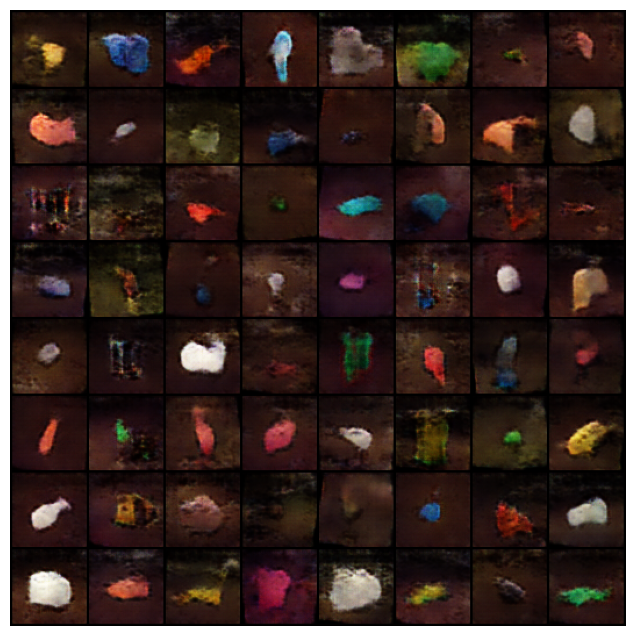
\includegraphics[scale=0.5]{./imgs/3epochs.png}
\end{center}
We assume that this is due to the variation between the legos is higher than the faces in celeba.


\noindent Due to the two issues above, we have 200k images and decided to raise the number 
of epochs to 40 and thus our hyperparameters are:
\begin{center}
\begin{tabular}{|c|c|}
\hline
& Params for our DCGAN \\ \hline
Resolution & 64x64x3 \\ \hline
Latent Space Dim & 100 \\ \hline
Epochs & 40 \\ \hline
Learning Rate & 0.0002 \\ \hline
Beta1 (Adam) & 0.5 \\ \hline
Batch Size & 128 \\ \hline
\end{tabular}
\end{center}


\subsubsection*{Issue: Resolution}
We tried changing the dimensions of the data to a higher resolution but we couldn't resolve some immediate errors that occurred relating
to the dimensions of some vector. Thus the resolution was kept at 64x64.

\subsubsection*{Issue: Seeding}
Heres the order of operations:
$$
\text{Seeding}
\rightarrow
\text{Training dataset augmentation and creation}
\rightarrow
\text{Fixed noise}
\rightarrow \dots
$$

\noindent This fixed noise was used to keep track of how the legos turned
out over time and since the dataset batching and augmentation happened before
the fixed noise, when trying to load the trained model, the fixed noise would look
different without the training dataset. The easy fix would be to change the order
at which it happens:
$$
\text{Seeding}
\rightarrow
\text{Fixed noise}
\rightarrow
\text{Training dataset augmentation and creation}
\rightarrow \dots
$$
\newpage
\subsubsection*{Takeaways}
\begin{itemize}
    \item Keep track of both the discriminator and generator. Getting a checkpoint of the model at some location is a good decision. There are many times when the discriminator or generator wins over the other and drives the model off the cliff. Sometimes it is generally hard to avoid the wrong gradient step for both models, thus having checkpoints and going back to that gives a good impression of what happened at that iterative step. Moreover, you can recover a model from taking the wrong step as well by saving checkpoints.  \\
    \item We noticed that adding noise to the background helped the results. Originally we had a white background, and was able to generate the following with 100 epochs (left image). Compared to the new images we generated (right image), the original images performed worse on our GAN. \\ \\ \\
    \hspace*{-1.5cm}
    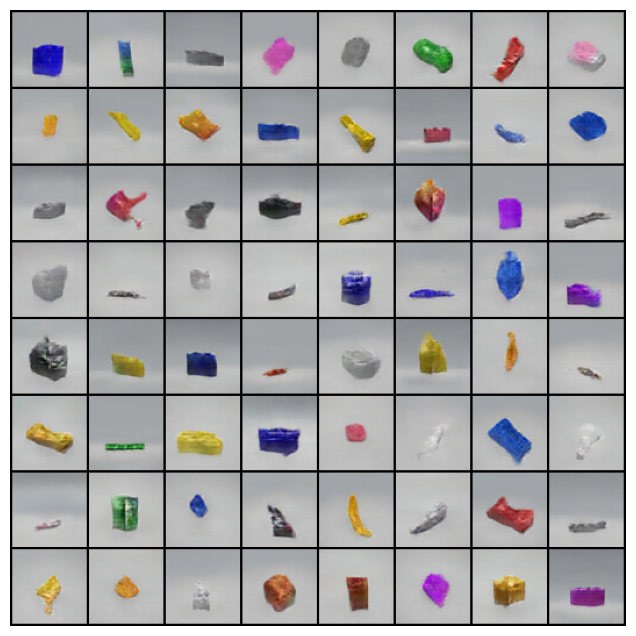
\includegraphics[scale = 0.4]{imgs/100 epoch gan.png}
    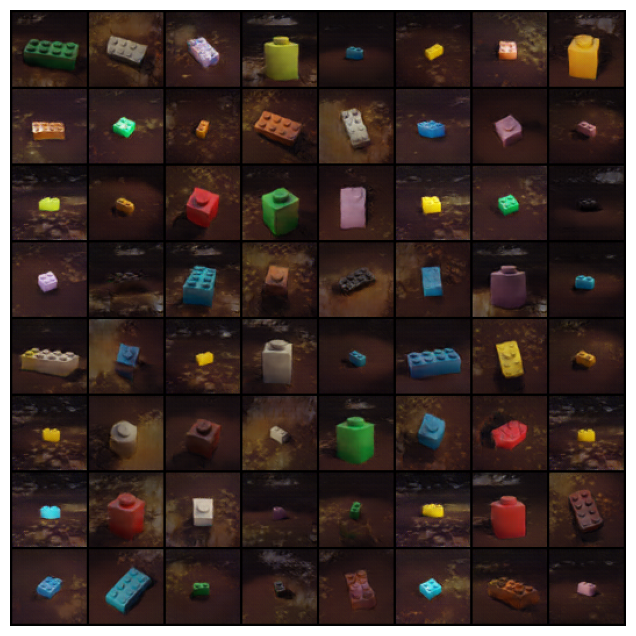
\includegraphics[scale = 0.4]{imgs/gan bricks only.png}
\end{itemize}

\newpage
\subsection*{b. Example Images}
These are generated with the new dataset of legos (200k images with colorful background + 200k augmented images).
\begin{center}
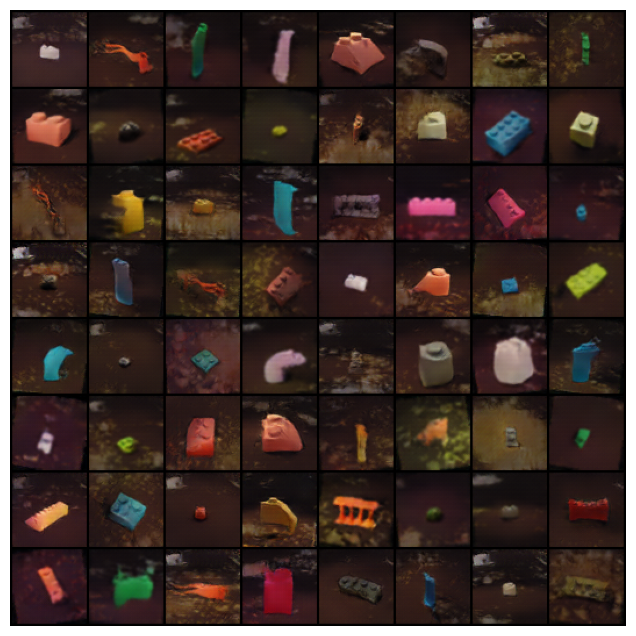
\includegraphics[scale=0.65]{imgs/gan with augmentation.png}
\end{center}

With the GAN theres seems to be a lot of legos that are miscolored with multiple colors. Compared to the VAE dataset, the GAN also had more trouble with properly defining the edges of the Legos. \\

\subsection*{More Example Images}
\begin{center}
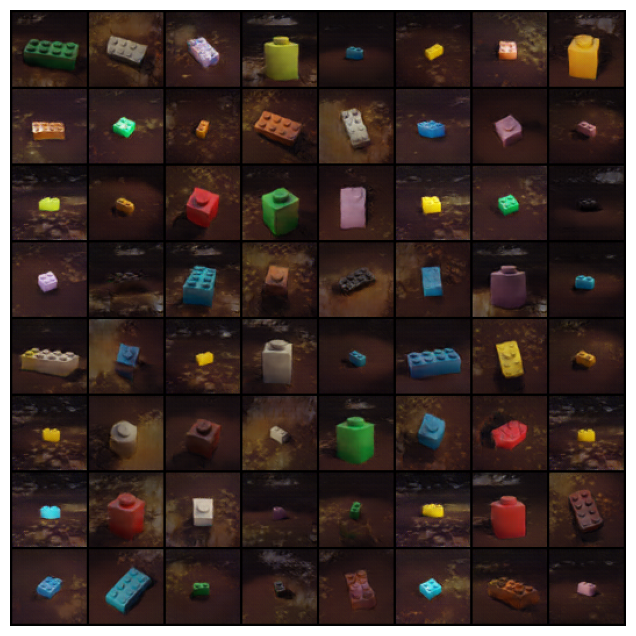
\includegraphics[scale=0.65]{imgs/gan bricks only.png}
\end{center}
These are only the lego bricks class, since it's a much narrower selection of shapes, the GAN results are able to generate much more realstic results with more accurate edges.

\newpage
\noindent We also decided to train a DCGAN on the VAE dataset to compare:
\begin{center}
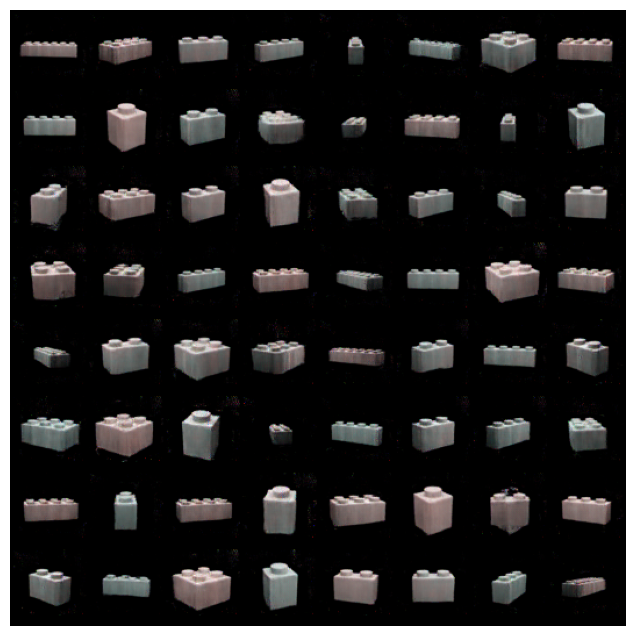
\includegraphics[scale=0.75]{./imgs/gan_vae}
\end{center}
These legos have much more defined studs and edges as compared to the VAE legos however, like the above result there are legos that have multiple colors and there is still a bunch
of noise that is discoloring the legos.


\newpage


\subsection*{c1. Interpolation}
Here is an interpolation between 4 different latent vectors:
\begin{center}
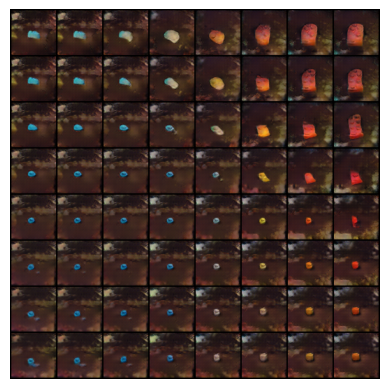
\includegraphics[scale=1.2]{./imgs/gan_interp_aug}
\end{center}

\newpage
\subsubsection*{Issue: Lego Inconsistency}
Interpolating between these 4 legos gave us legos that weren't the same as the input ones
(see the bottom left is green tipped instead of pink tipped):
\begin{center}
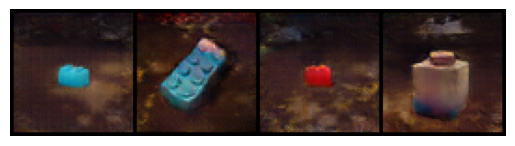
\includegraphics[scale=0.75]{./imgs/seed_69,0,23,42,62_legos}
\end{center}

\begin{center}
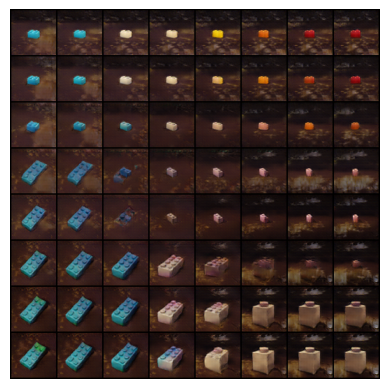
\includegraphics[scale=1]{./imgs/seed_69,0,23,42,62_wrong}
\end{center}

The network takes a $B$ (batch) sized of vector of latents and
converts it to batch of images
$$
(B \times d_z \times 1 \times 1)
\rightarrow_{G}
(B \times 3 \times 64 \times 64)
$$
The fix was to individually send each image through the network and combine the images
afterwards: 
$$
(1 \times d_z \times 1 \times 1)
\rightarrow_{G}
(1 \times 3 \times 64 \times 64)
$$

\begin{center}
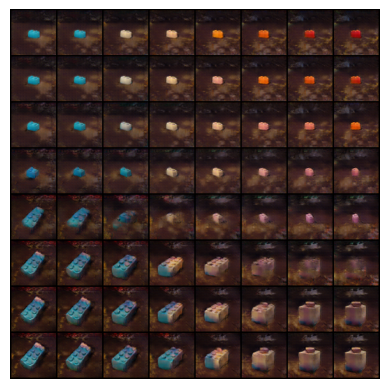
\includegraphics[scale=1.2]{./imgs/seed_69,0,23,42,62_interpolation}
\end{center}
As you can see the bottom left lego is now pink tipped instead of green tipped.

\subsection*{c2. Interpolation Video}
Generating many different latent vectors and interpolating between them in a video. See Box or Github for the mp4 file.
% TODO LINK
\begin{center}
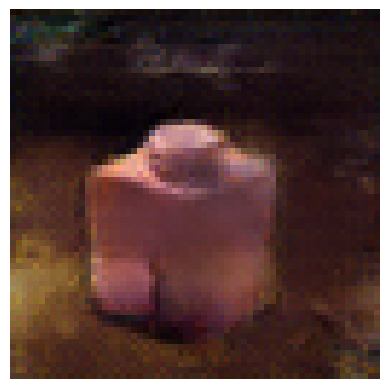
\includegraphics[scale=0.25]{./imgs/f1}
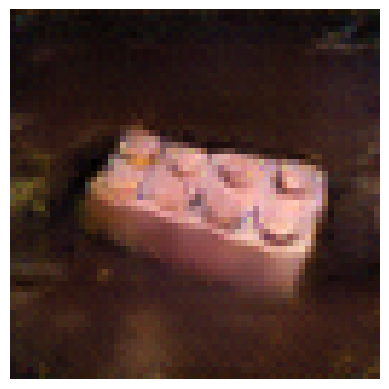
\includegraphics[scale=0.25]{./imgs/f2}
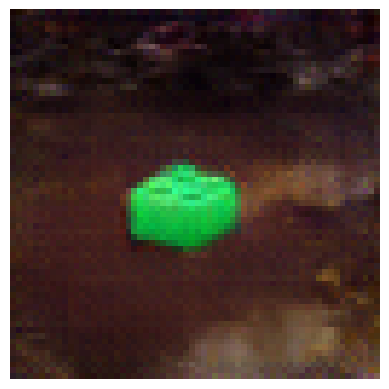
\includegraphics[scale=0.25]{./imgs/f3}
\end{center}

\newpage
\subsection*{c3. Adding Constants to Latents}
I was interested to see what happened if I continuously added a constant to the latent space and do it for 8 steps.
The legos start to morph to different legos as expected but
they all eventually end up at a terminal lego when the floats in the latent gets too big:
\begin{center}
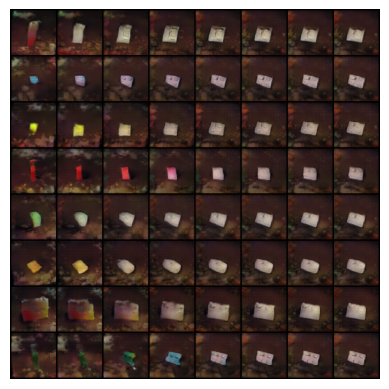
\includegraphics[scale=1.5]{./imgs/gan_adding_constants}
\end{center}

\newpage
\section*{Problem 3: Diffusion Models}
\subsection*{a. Architecture and Hyperparamters}
We used a \href{https://arxiv.org/pdf/2006.11239.pdf}{Denoising Diffusion Probabilistic Model (DDPM)}. The original hyperparameters for
the \href{https://github.com/lucidrains/denoising-diffusion-pytorch}{DDPM repo} that we used were:
\begin{center}
\begin{tabular}{|c|c|}
\hline
& Params for repo DDPM \\ \hline
Resolution & 128x128x3 \\ \hline
Time Steps & 1000 \\ \hline
Training Steps & 700k \\ \hline
Learning Rate & 8e-5 \\ \hline
Ema Decay & 0.995 \\ \hline
Gradient Accumulate Every & 2 \\ \hline
\end{tabular}
\end{center}

\noindent We decided to keep the resolution the same as the GAN to
keep comparisons more fair. The only hyperparameter that we changed was
the training steps since 700k was going to take way too long
and 10k gave good results already. The model took us around 5 hours to train from scratch.

\begin{center}
\begin{tabular}{|c|c|}
\hline
& Params for repo DDPM \\ \hline
Resolution & 64x64x3 \\ \hline
Time Steps & 1000 \\ \hline
Training Steps & 20k \\ \hline
Learning Rate & 8e-5 \\ \hline
Ema Decay & 0.995 \\ \hline
Gradient Accumulate Every & 2 \\ \hline
\end{tabular}
\end{center}

\subsubsection*{Issue: Augmentation}
We Realized that the diffusion model has its own Dataloader inside the pip package and thus we were
not able to apply the augmentations directly to the tensors when they were loaded in. Thus this diffusion model was trained without the augmented images.


\subsubsection*{Issue: Taking to long to train}
Started training the DDPM without changing the hyperparameters and it was 2k/700k steps in and it had taken 5 hours.
The reason why it was taking so long was because it was doing FID Evaluations: they would take forever
since each image had 250 timesteps and there were 1500 evaluations.
I calculated that would it would take approx 60 days to train with evaluations. The fix was to
just turn off the evaluations by setting it to False.

\subsection*{Takeaways}
\begin{itemize}
    \item If you are using a prebuilt library for your diffusion model, do more research of what your model is actually doing in code so that you can more easily modify what it is doing to suit what you want to achieve.
\end{itemize}

\newpage
\subsection*{b. Example Images}
Here is 25 images sampled randomly from the latent space:
\begin{center}
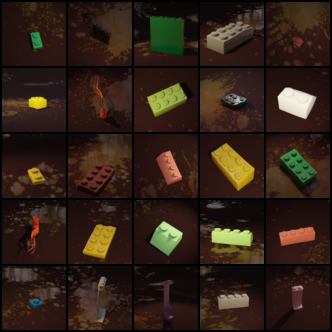
\includegraphics[scale=1]{./imgs/25_diff}
\end{center}
The diffusion model picked up the defined hard edges of a lego, the studs,
the correct number of studs for the blocks (usually) and the characteristics of the different classes (slopes, walls, plates, bricks).
The images are very reasonable and most of them would pass for actual legos.
Compared to the GAN generated images, the legos are more well defined 
than the GAN's: the edges and much sharper, and there are consistent colors for the pieces. 

\newpage
\subsection*{More Example Images}
Like the GAN section, here is a diffusion model trained on the dataset we used for the VAE: \\
\begin{center}
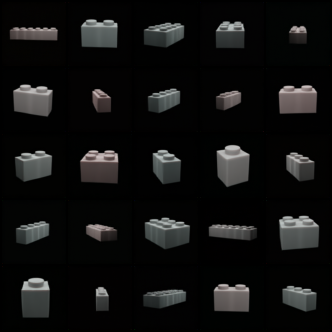
\includegraphics[scale=1]{./imgs/25_diff_vae}
\end{center}

\noindent Same conclusion as the one on the new dataset but this time the model managed to capture the rendering issues present in between the studs.

\subsubsection*{Issue: VRAM Issues}
I was running out of VRAM when generating more than 5 images at a time. The fix was to
generate one image at a time, bring it to CPU/RAM and clear the cache in the GPU.
\newpage
\subsection*{c1. Interpolation}
Here is an interpolation between two different latent spaces:
\begin{center}
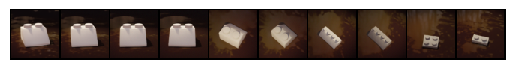
\includegraphics[scale=1.3]{./imgs/interp_diff}
\end{center}
Compared to the GAN and VAE, the interpolation between different bricks happens very suddenly.
There isn't really good in between bricks, which makes since since the diffusion model generates very well defined images of the legos. \\ \\
Just like the GAN, here is an interpolation between four different latent spaces:
\begin{center}
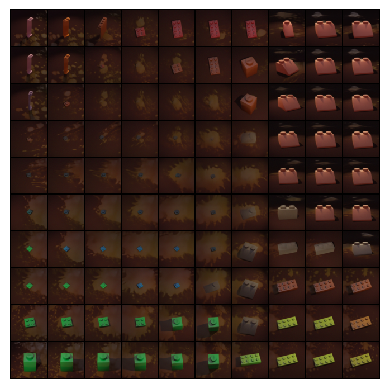
\includegraphics[scale=1.5]{imgs/diffusion_interp_between_4.png}
\end{center}
\newpage
\subsection*{c2. Interpolation Video}
As with the GAN we created a video of the interpolation between many different latent spaces on Box and Github.


\end{document}  